\documentclass[11pt,a4paper]{article}
\usepackage[margin=2.2cm]{geometry}
\usepackage{fontspec}
\setmainfont{Palatino}
\setmonofont{Menlo}[Scale=0.82]
\newfontfamily\ipafont{Times New Roman}
\usepackage{graphicx,booktabs,array,xcolor,caption,enumitem,float}
\usepackage[section]{placeins}
\usepackage{tikz}
\usetikzlibrary{positioning,arrows.meta}
\usepackage[hidelinks]{hyperref}
\hypersetup{pdftitle={Forced Alignment with the Montreal Forced Aligner}, pdfauthor={Srivardhan Ginjala}}
\graphicspath{{figures/}}
\captionsetup{font=small,labelfont=bf,labelsep=period,skip=6pt}
\captionsetup[table]{position=top}
\setlist{itemsep=2pt,topsep=4pt}
\renewcommand{\topfraction}{0.85}
\renewcommand{\bottomfraction}{0.6}
\renewcommand{\textfraction}{0.1}
\renewcommand{\floatpagefraction}{0.85}
\newcommand{\code}[1]{\texttt{#1}}
\newcommand{\ph}[1]{\texttt{/#1/}}
\newcommand{\ipa}[1]{{\ipafont /#1/}}
\newcommand{\repo}{gsri-18/MFA-Alignment-and-Multimodal-Emotion-Recognition}
\renewcommand{\arraystretch}{1.2}
\setlength{\emergencystretch}{2em}
\definecolor{blk}{HTML}{E8EEF7}
\definecolor{blkb}{HTML}{4A6FA5}
\tikzset{
  stage/.style={draw=blkb, fill=blk, rounded corners=2pt, align=center, font=\small,
                text width=2.45cm, minimum height=1.35cm, inner sep=3pt},
  arr/.style={-{Stealth[length=2.2mm]}, thick, draw=black!70},
}

\title{\textbf{Forced Alignment with the Montreal Forced Aligner}\\[2pt]\large Assignment 2a Report}
\author{Srivardhan Ginjala}
\date{November 2026}

\begin{document}
\maketitle

\begin{center}\small
The code, TextGrids and figures are at \href{https://github.com/\repo}{\texttt{github.com/\repo}}.
\end{center}

\begin{abstract}
\noindent I aligned the six provided clips with the Montreal Forced Aligner (MFA) 3.4.4 and compared two pretrained
acoustic models, three pronunciation dictionaries and a speaker-adapted model. One script runs the whole pipeline,
from the raw audio to TextGrids, checks and figures. With the \code{english\_us\_arpa} model every word matches its
transcript. Changing the dictionary or adapting the model moves the word boundaries by less than one 10~ms frame on
average. The \code{english\_mfa} model agrees closely on the news reader but fails on two learner clips, where the
final consonant runs on for about two seconds of trailing audio.
\end{abstract}

%=====================================================================
\section{Data and pipeline}

The data are three BU Radio News paragraphs read by one news reader (25 to 31~s each) and three short sentences from
the ISLE corpus in which a learner of English reads minimal pairs (``I said white not bait''). The 244 word tokens
contain 151 distinct words. \code{Assignment\_2a/align.py} runs the five stages in Figure~\ref{fig:pipeline}, and the
Colab notebook in \code{colab/} ran them on a CPU runtime in 7.4 minutes, including the MFA install.

\begin{figure}[htbp]
\centering
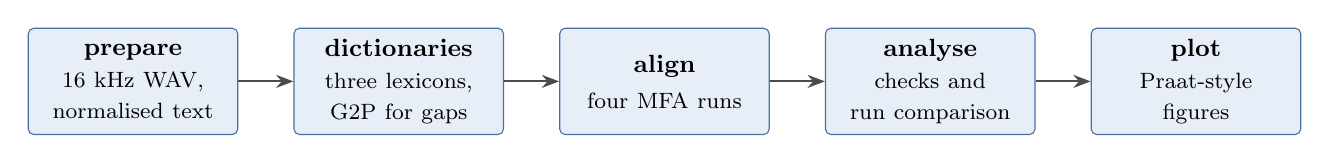
\begin{tikzpicture}[node distance=7mm]
  \node[stage] (p) {\textbf{prepare}\\[2pt]\footnotesize 16 kHz WAV,\\normalised text};
  \node[stage, right=of p] (d) {\textbf{dictionaries}\\[2pt]\footnotesize three lexicons,\\G2P for gaps};
  \node[stage, right=of d] (a) {\textbf{align}\\[2pt]\footnotesize four MFA runs};
  \node[stage, right=of a] (n) {\textbf{analyse}\\[2pt]\footnotesize checks and\\run comparison};
  \node[stage, right=of n] (f) {\textbf{plot}\\[2pt]\footnotesize Praat-style\\figures};
  \draw[arr] (p) -- (d); \draw[arr] (d) -- (a); \draw[arr] (a) -- (n); \draw[arr] (n) -- (f);
\end{tikzpicture}
\caption{The alignment pipeline. Each stage also runs alone with \code{--stage}.}
\label{fig:pipeline}
\end{figure}

Three clips are NIST SPHERE files, so every clip is converted to 16~kHz RIFF WAV. Each speaker gets a folder so that
MFA adapts to the two voices separately. Table~\ref{tab:norm} shows how the transcripts become the spoken words.

\begin{table}[htbp]
\centering\small
\caption{Transcript normalisation.}
\label{tab:norm}
\begin{tabular}{lll}
\toprule
Transcript & Aligned as & Reason \\
\midrule
\code{S.J.C.'s} & \code{s j c's} & read letter by letter \\
\code{WBUR's} & \code{w b u r's} & a call sign, read letter by letter \\
\code{seventy- six}, \code{de-politicize} & \code{seventy six}, \code{de politicize} & hyphens split words \\
punctuation, capitals & removed, lower case & the lexicons are lower case \\
\bottomrule
\end{tabular}
\end{table}

%=====================================================================
\section{Dictionaries and acoustic models}

Table~\ref{tab:runs} lists the four alignments. Each lexicon covers exactly the corpus words. The \code{arpa} and
\code{mfa\_ipa} lexicons take the pretrained entries and fill the missing words with the matching MFA G2P model. The
\code{g2p\_en} lexicon uses the builder from my earlier FastSpeech~2 assignment, which takes every CMUdict variant and
the g2p\_en neural G2P for words CMUdict lacks. All model versions are pinned. The \code{english\_mfa} dictionary stays
at 3.0.0 because its 3.1.0 release holds a reduced lexicon with Indian English phones.

\begin{table}[htbp]
\centering\small
\caption{The four alignments, all with \code{--beam 100 --retry\_beam 400}.}
\label{tab:runs}
\begin{tabular}{lllc}
\toprule
Run & Acoustic model & Lexicon source & Words from G2P \\
\midrule
\code{arpa} (reference) & \code{english\_us\_arpa} 3.0.0 & \code{english\_us\_arpa} dictionary & 4 \\
\code{g2p\_en} & \code{english\_us\_arpa} 3.0.0 & CMUdict through g2p\_en & 3 \\
\code{mfa\_ipa} & \code{english\_mfa} 3.1.0 & \code{english\_mfa} dictionary 3.0.0 & 9 \\
\code{arpa\_adapted} & \code{english\_us\_arpa}, adapted & \code{english\_us\_arpa} dictionary & 4 \\
\bottomrule
\end{tabular}
\end{table}

%=====================================================================
\section{Results}

Every run aligned all six clips, and every word tier matches the normalised transcript with no unknown-word phones.
Table~\ref{tab:checks} sums the automatic checks. A phone of 30~ms or less (three 10~ms frames, and two \code{arpa} phones
last only 10~ms) usually marks a sound the speaker reduced. A speech phone over 250~ms usually contains a pause or noise.

\begin{table}[htbp]
\centering\small
\caption{Automatic checks. MFA's speech log likelihood is per frame, averaged over the six clips, and is comparable only
between runs of the same acoustic model.}
\label{tab:checks}
\begin{tabular}{lccccc}
\toprule
& & & \multicolumn{2}{c}{Phones over 250 ms} & \\
\cmidrule(lr){4-5}
Run & News reader phones & 30 ms or less & News reader & Learner & Speech log likelihood \\
\midrule
\code{arpa} & 1{,}025 & 82 (8.0\%) & 1 & 1 & $-47.77$ \\
\code{g2p\_en} & 1{,}025 & 79 (7.7\%) & 1 & 1 & $-47.74$ \\
\code{mfa\_ipa} & 1{,}008 & 106 (10.5\%) & 4 & 4 & $-44.92$ \\
\code{arpa\_adapted} & 1{,}025 & 82 (8.0\%) & 1 & 1 & $-46.77$ \\
\bottomrule
\end{tabular}
\end{table}

\begin{table}[htbp]
\centering\small
\caption{Boundary shifts against the \code{arpa} run in ms, averaged over each speaker's clips. Phone shifts are not
defined for \code{mfa\_ipa}, which uses a different phone set.}
\label{tab:diff}
\begin{tabular}{llcccc}
\toprule
& & \multicolumn{3}{c}{Word boundaries} & Phone boundaries \\
\cmidrule(lr){3-5}\cmidrule(lr){6-6}
Run & Speaker & Mean shift & Largest shift & Over 50 ms & Mean shift \\
\midrule
\code{g2p\_en} & news reader & 0.2 & 30 & 0\% & 0.2 \\
 & learner & 0 & 0 & 0\% & 0.3 \\
\code{arpa\_adapted} & news reader & 0.1 & 10 & 0\% & 0.1 \\
 & learner & 0 & 0 & 0\% & 0 \\
\code{mfa\_ipa} & news reader & 8.3 & 250 & 2.4\% & n/a \\
 & learner & 175 & 2{,}460 & 23\% & n/a \\
\bottomrule
\end{tabular}
\end{table}

%=====================================================================
\section{Sample alignments}

The figures show Praat's analysis through parselmouth (waveform, spectrogram, F0) with the word and phone tiers below,
as in Praat's TextGrid editor. Labels of the shortest phones are left out where they would overlap.

\begin{figure}[htbp]
\centering
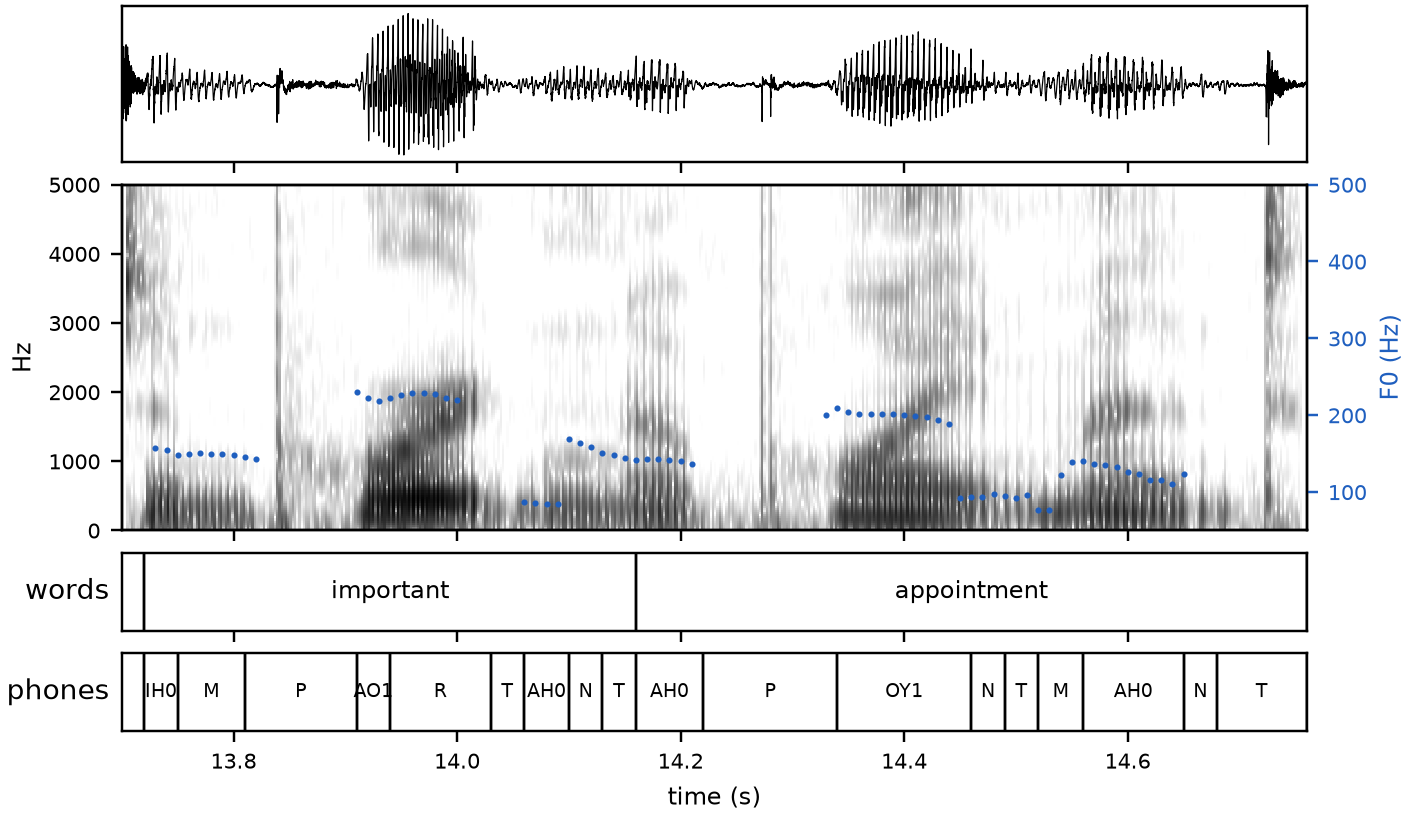
\includegraphics[width=0.92\textwidth]{a2a_bu_important.png}
\caption{F2BJRLP1, \textit{important appointment} (13.70 to 14.76~s), \code{arpa} run. In \textit{important} the final \ph{T AH0 N T} spans 130~ms, and
three of its four phones last 30~ms. In \textit{appointment} the \ph{N T} of the second syllable gets 30~ms each.}
\label{fig:bu}
\end{figure}

\begin{figure}[htbp]
\centering
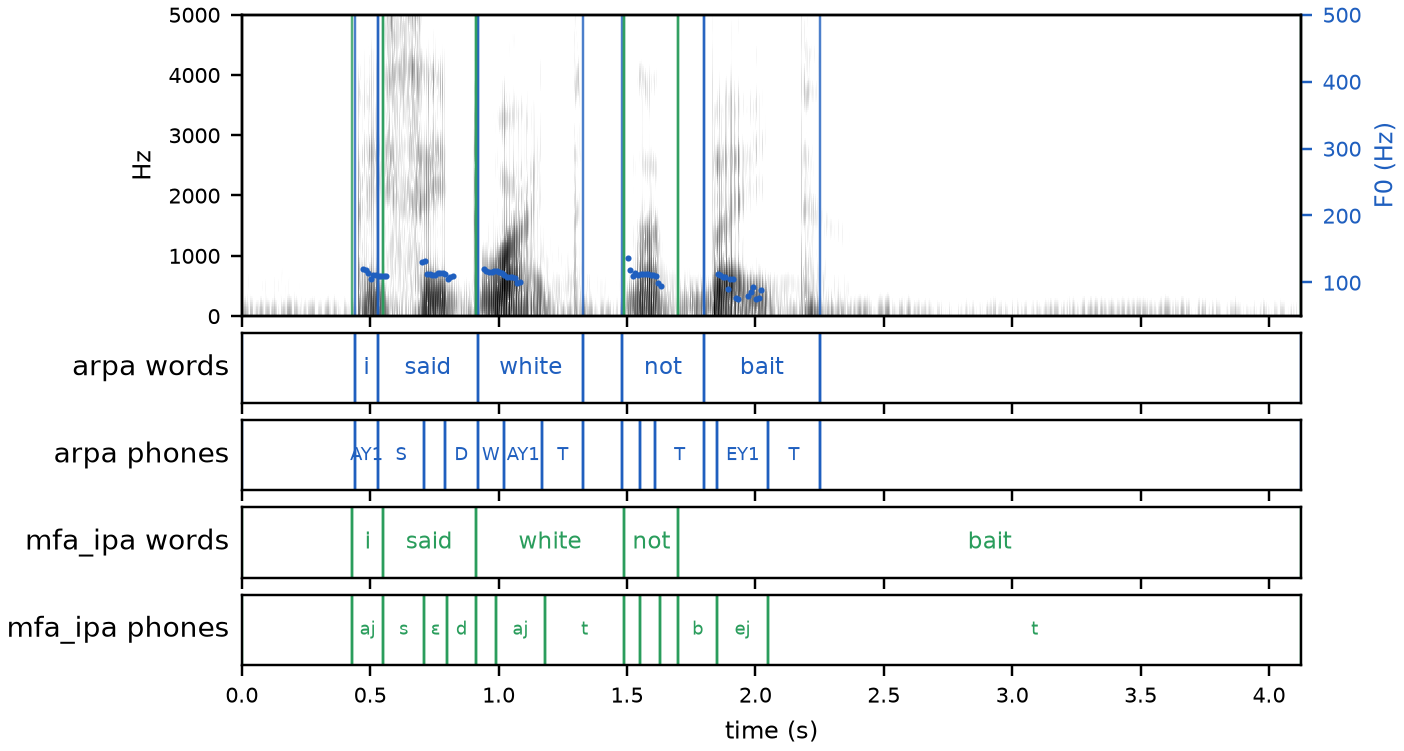
\includegraphics[width=0.92\textwidth]{a2a_isle_runs.png}
\caption{``I said white not bait'' aligned by the \code{arpa} run (blue) and the \code{mfa\_ipa} run (green). The
\code{arpa} run ends \textit{bait} at the release of its \ph{T} (2.25~s). The \code{mfa\_ipa} run stretches that
\ipa{t} to the end of the recording.}
\label{fig:isle}
\end{figure}

%=====================================================================
\section{Observations}
\begin{itemize}
\item \textbf{The news reader aligns cleanly.} In the figures I inspected, the boundaries fall on onsets, releases and
  formant changes, and the 31 pauses inside the paragraphs (7.5~s in all) come out as silences.
\item \textbf{Short phones mark reductions.} Almost half of the phones of 30~ms or less are \ph{T}, \ph{N} and
  \ph{AH0} (37 of 82), often in clusters such as the \ph{T AH0 N T} of \textit{important} (Figure~\ref{fig:bu}). The
  dictionary forces the full form, so the sounds the reader reduced get the shortest time allowed. The one long phone of
  the news reader is the phrase-final \ph{OW1} of \textit{ago} before a comma (290~ms).
\item \textbf{The dictionary barely matters.} The \code{arpa} and \code{g2p\_en} runs share CMUdict pronunciations.
  Their word boundaries differ by at most 30~ms and their phone boundaries by at most 50~ms.
\item \textbf{G2P errors are visible.} The MFA G2P gives \textit{dukakis} a stressed \ph{UW1} in the \code{arpa}
  lexicon, and that vowel gets only 30~ms in F2BJRLP1. CMUdict, which \code{g2p\_en} uses, has the unstressed
  \ph{UW0}. The IPA G2P drops the vowel of spelled letters, turning \textit{c's} into \ipa{kʰ z} and \textit{r's} into
  \ipa{ɹ z}, while the ARPAbet dictionary contains both words.
\item \textbf{Adaptation barely moves the boundaries.} It improves the speech log likelihood by about one unit per frame. Word
  boundaries move by at most one frame and phone boundaries by at most 30~ms.
\item \textbf{The \code{english\_mfa} model fails on the learner.} On the news reader its word boundaries are 8~ms from
  those of the \code{arpa} run on average. On two learner clips the final \ipa{t} of \textit{bait} and \ipa{d} of
  \textit{bed} run on 1.9 and 2.5~s past the point where the \code{arpa} run ends those words. A possible cause is that
  its silence model does not match the faint background noise.
\item \textbf{Forced alignment cannot detect mispronunciation.} The aligner always labels the dictionary's phones, so
  \textit{bait} gets \ph{EY1} whatever vowel the learner produced. Detecting it needs free phone recognition or a
  goodness of pronunciation score.
\item \textbf{Repeated runs differ slightly.} A local test run and the Colab run differ by one frame at a few
  boundaries.
\end{itemize}

%=====================================================================
\section{Extra credit and reproducibility}
\begin{itemize}
\item \textbf{Custom lexicons.} Each lexicon is built for the corpus words. Two fill the gaps in pretrained dictionaries
  with MFA's pretrained G2P models, and the third uses CMUdict with the g2p\_en neural G2P. No G2P model was trained.
\item \textbf{Several acoustic models.} Two pretrained acoustic models, \code{english\_us\_arpa} and
  \code{english\_mfa}, and a speaker-adapted copy of the first.
\item \textbf{Automation.} \code{python align.py} runs everything. The Colab notebook installs MFA, runs the script and
  saves the outputs, the executed notebook and the logs by itself.
\item \textbf{Reproducibility.} \code{Assignment\_2a/README.md} gives the setup and commands. The provided audio is
  licensed, so it is not in the repository.
\end{itemize}

\end{document}
